\section{Jakościowe porównanie algorytmów}

Filtry przygotowane przez 4 zespoły zostały porównane pod względem jakości filtracji. Autorzy na etapie implementowania filtrów testowali swoje algorytmy pod kątem usuwania szumów wysokiej częstotliwości, a zatem wygładzania sygnału.

W celu sprawdzenia jak przygotowane filtry wpływają na sygnał, zostały wyznaczone: widmowa gęstość mocy sygnału EKG przed i po filtracji oraz błąd średniokwadratowy rozumiany jako różnica między sygnałem oryginalnym i odfiltrowanym. Testy były przeprowadzane na sygnale testowym z bazy MIT-BIH o numerze 100.

\subsection{Widmowa gęstość mocy}

Widmowa gęstość mocy (PSD) pozwala zobaczyć, które częstotliwości przenoszą największą energię w sygnale. PSD została wyznaczona na podstawie periodogramów wcześniej zebranych wyjść poszczególnych algorytmów.

Na wykresach gęstości mocy można zauważyć, które częstotliwości są usuwane przez filtr. Dzięki temu zyskujemy informację o typie zakłócenia, które możemy wygasić używając algorytmu o przyjętych parametrach.

Na rysunkach \ref{rys:emd}, \ref{rys:emd2}, \ref{rys:wwf}, \ref{rys:nlm}, \ref{rys:sg} przedstawiono skutki użycia zaimplementowanych algorytmów w roli filtrów dolnoprzepustowych. 

\begin{figure}[H]
  \begin{center}
    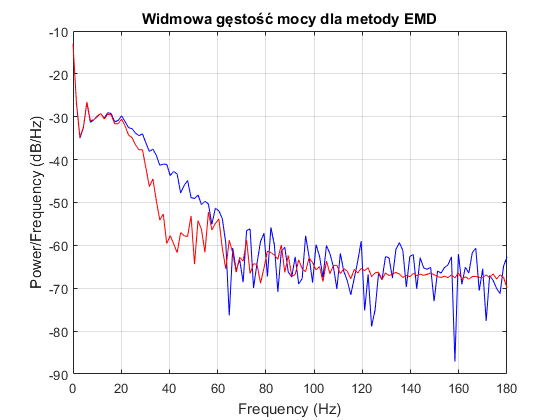
\includegraphics[scale=0.9]
    {img/emd_psd_250.png}
  \end{center}
  \caption{Widmowa gęstość mocy sygnału EKG oraz sygnału przefiltrowanego metodą EMD z usuniętą 1 składową IMF}
  \label{rys:emd}
\end{figure}

\begin{figure}[H]
  \begin{center}
    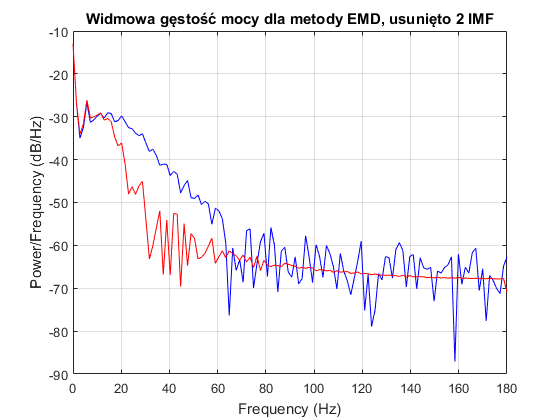
\includegraphics[scale=0.9]
    {img/PSD_EMD_2discarded.png}
  \end{center}
  \caption{Widmowa gęstość mocy sygnału EKG oraz sygnału przefiltrowanego metodą EMD z usniętymi 2 składowymi IMF}
  \label{rys:emd2}
\end{figure}

\begin{figure}[H]
  \begin{center}
    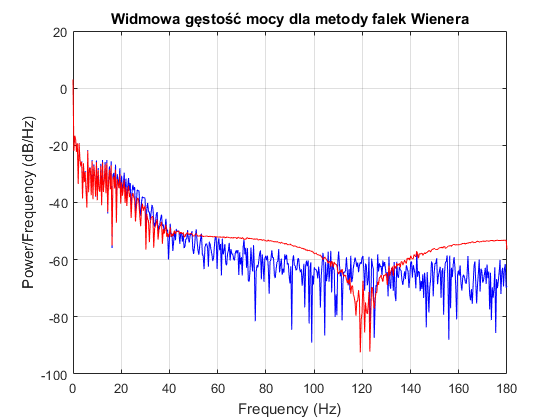
\includegraphics[scale=0.9]
    {img/PSD_WWF1.png}
  \end{center}
  \caption{Widmowa gęstość mocy sygnału EKG oraz sygnału przefiltrowanego metodą WWF, TM = 1, dekompozycja do 3 poziomu, rozmiar okna mediany = 201}
  \label{rys:wwf}
\end{figure}

\begin{figure}[H]
  \begin{center}
    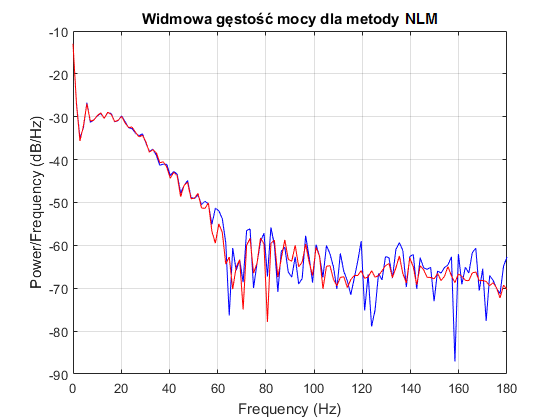
\includegraphics[scale=0.9]
    {img/PSD_NLM_250.png}
  \end{center}
  \caption{Widmowa gęstość mocy sygnału EKG oraz sygnału przefiltrowanego metodą NLM, otoczenie P = 10, połowa sąsiedztwa M = 2000}
  \label{rys:nlm}
\end{figure}

\begin{figure}[H]
  \begin{center}
    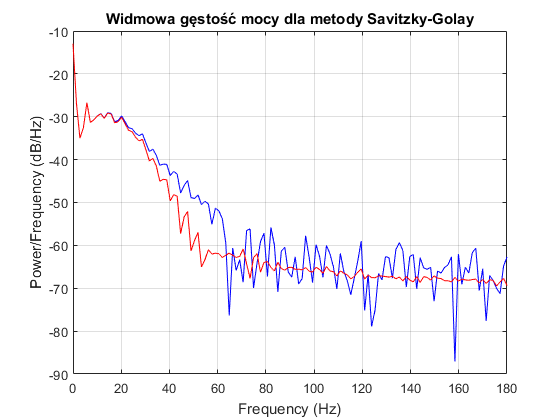
\includegraphics[scale=0.9]
    {img/PSD_SG_M5.png}
  \end{center}
  \caption{Widmowa gęstość mocy sygnału EKG oraz sygnału przefiltrowanego metodą SG, interpolacja wielomianem stopnia 2, szerokość okna 11 próbek}
  \label{rys:sg}
\end{figure}

Możliwa jest również filtracja górnoprzepustowa, czyli usunięcie szumów o niskiej częstotliwości. Gęstość mocy filtra SG do wykrywania i usuwania składowych wolnozmiennych przedstawia rysunek \ref{rys:sg1}.

\begin{figure}[H]
  \begin{center}
    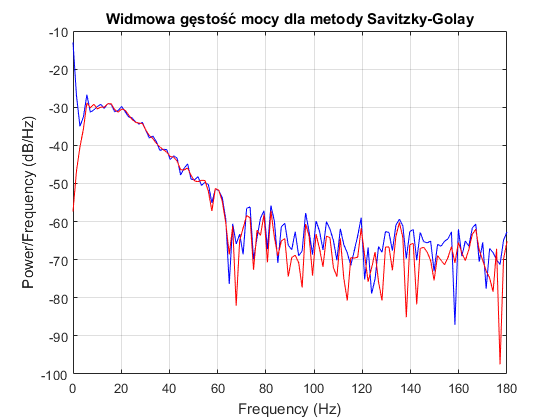
\includegraphics[scale=0.9]
    {img/PSD_SG_M50.png}
  \end{center}
  \caption{Widmowa gęstość mocy sygnału EKG oraz sygnału, gdzie metodą SG odrzucono szum o niskiej częstotliwości, interpolacja wielomianem 2 stopnia, długość ramki 101 próbek}
  \label{rys:sg1}
\end{figure}


\subsection{Dyskusja zakłóceń w dziedzinie częstotliwości}

Aby ocenić metody pod kątem przydatności, należy podać informacje na temat typowych zakłóceń, które utrudniają pracę z sygnałem EKG. Są to m.in.: zakłócenia od sieci energetycznej, zmiany oporności kontaktu elektroda-skóra, artefakty pochodzące od ruchów i oddechu pacjenta i sprzężenia od EMG \cite{Djordje}.

W tabeli \ref{tab:noise} zebrano typy zakłóceń EKG wraz z ich możliwymi zakresami częstotliwości.

\begin{table}[!htbp]
  \centering
  \begin{tabular}{|c|c|c|c|}
  \hline 
  Zakłócenie & Pasmo \\  
  \hline 
  Szum zasilania & 50 lub 60 Hz i harmoniczne \\
  \hline
  Zmiana rezystancji elektroda-skóra & \textless 0,5 Hz \\
  \hline
  Oddychanie pacjenta &  0,15 - 0,3 Hz \\
  \hline
  Ruchy pacjenta & \textless 0,5 Hz \\
  \hline
  Szum elektromiogramu & 20 - 1000 Hz \\
  \hline
\end{tabular} 
\caption{Pasma typowych zakłóceń w sygnale EKG}
\label{tab:noise}
\end{table}

Jeżeli za użyteczny zakres sygnału EKG przyjmiemy częstotliwości 0,5 - 50 Hz, to możemy ocenić użycie metod z wybranymi przez autorów parametrami. Filtracja metodą \textbf{NLM} najbardziej zachowuje przetwarzany sygnał. Osłabieniu ulegają tylko częstotliwości w okolicy 60Hz, co może posłużyć do usuwania wpływu linii zasilającej w niektórych państwach. Obcinana częstotliwość zależy od przyjętych parametrów algorytmu, lecz ze względu na jego długie działanie nie została przeprowadzona dokładna analiza ich wpływu na widmo sygnału wyjściowego.

Metody EMD i Savitzky-Golay zachowują się jak filtry dolnoprzepustowe. Metoda \textbf{EMD} przy badanych parametrach wygasza najbardziej częstotliwości od 40 Hz, jednak osłabienie zaczyna się już od 20 Hz. Na rysunku \ref{rys:emd2} widać, że odrzucenie dwóch składowych IMF obcina pasmo poczynając od jeszcze niższej częstotliwości. Daje to podstawy aby użyć filtra EMD również do usuwania artefaktów ruchu, oddychania czy poruszeń elektrod, jeśli usunie się więcej składowych IMF, a następnie odejmie wynik od oryginalnego sygnału.

Algorytm \textbf{Savitzky-Golay} dla okna o szerokości 11 próbek wygasza częstotliwości powyżej 50 Hz i zauważalnie osłabia składowe powyżej 30 Hz. Jeśli użyje się szerszego okna, dane są wygładzane mocniej i są usuwane też pasma o niższej częstotliwości. Na rysunku \ref{rys:sg1} przedstawiono przykład użycia filtru SG z oknem o szerokości 101 próbek do usunięcia zakłóceń wolnozmiennych poniżej 3 Hz. Z kolei przy ramce długości 1201 próbek zaobserwowano obcięcie szumów poniżej 1 Hz.

Metoda falek Wienera \textbf{WWF} przy badanych parametrach zadziałała jak filtr pasmowo-zaporowy usuwając składowe 115-125 Hz. Metoda nie wpłynęła znacząco na pasmo 0-40Hz. Odpowiedni dobór parametrów pozwala na usunięcie szumów o znanej częstotliwości, np. zakłócenia linii zasilającej 50 Hz.

\subsection{Błąd średniokwadratowy}

Między sygnałami oryginalnymi i odfiltrowanymi został wyznaczony błąd średniokwadratowy (MSE). Zdecydowano się na takie rozwiązanie, ponieważ nie dla wszystkich metod znaleziono rozwiązania referencyjne (funkcje biblioteczne).

Parametr MSE wyznaczony między sygnałem oryginalnym i przetworzonym nie daje zatem informacji czy filtracja jest poprawna, ale pozwala ocenić, jak bardzo filtracja zmienia i zniekształca sygnał.

Wyniki analizy zostały zebrane w tabeli \ref{tab:mse}.


\begin{table}[!htb]
  \centering
  \begin{tabular}{|c|c|c|c|}
  \hline 
  Algorytm  & MSE \\  
  \hline 
  EMD, usunięto 1 IMF & 0,0015 \\
  \hline
  EMD, usunięto 2 IMF  & 0,0063 \\
  \hline
  EMD, usunięto 3 IMF  & 0.0115 \\
  \hline
  NLM, P = 10, M = 2000  & 6,9797e-5 \\
  \hline
  NLM, P = 5, M = 2000  & 7,0370e-5 \\
  \hline
  NLM, P = 5, M = 100  & 6,7657e-5 \\
  \hline
  WWF, rozmiar okna mediany = 201, poziom dekompozycji N = 3, TM = 1  & 0,0786 \\
  \hline
  WWF, rozmiar okna mediany = 201, poziom dekompozycji N = 2, TM = 1  & 0,0482 \\
  \hline
  SG, rozmiar okna M = 11, stopień wielomianu N = 2  & 3,4e-4 \\
  \hline
  SG, rozmiar okna M = 1001, stopień wielomianu N = 2  & 0,0283 \\
  \hline
  SG, rozmiar okna M = 41, stopień wielomianu N = 3  & 0,017 \\
  \hline
\end{tabular} 
\caption{Parametry filtru}
\label{tab:mse}
\end{table}

Po wykonaniu szeregu testów metod okazało się, że błąd średniokwadratowy pomiędzy sygnałem zaszumionym a odfiltrowanym nie jest parametrem przydatnym w analizie metod.

Dla algorytmu \textbf{WWF} poziom dekompozycji 2 z użyciem falek Haara mimo niższej wartości MSE poważnie zniekształcał już załamek T. Najlepsze rezultaty wygładzania, mimo nieco większego MSE dawał rozkład na falki do 3 poziomu. W przypadku algorytmu \textbf{EMD} zgodnie z oczekiwaniami widać, że dekompozycja i usunięcie każdej kolejnej funkcji składowej IMF coraz bardziej zniekształca sygnał. Metoda \textbf{NLM} nawet przy zmianach parametrów otoczenia i sąsiedztwa branego pod uwagę charakteryzuje się podobnym poziomem zniekształcenia podczas filtracji. Filtr \textbf{SG} charakteryzuje się niskim poziomem szumów, kiedy szerokość okna jest mała. Dla okna o szerokości 1001 próbek zniekształcenie jest bardzo duże, ponieważ jest to zestaw parametrów zupełnie wygładzający sygnał EKG i pozostawiający tylko izolinię.
